%!TeX root = main.tex
\section{Report of 2024 05 26}

I have spent the last couple of weeks solidifying the benchmarking/verification process. Section \ref{benchver}  is a full write up. It is probably important to read this since it shows - 1) The system has been tested in detail for accuracy, 2) the common benchmarking and reporting scheme. This will help to forstall any embarrassment over performance claims.

I have tested the system in three parts. One with no compute pipeline and one with both the compute and vertex pipelines active. The compute pipeline performance is the difference between the total and the graphics. Table \ref{tab:rccdPerfData1} is the graphics pipeline performance, table \ref{tab:rccdPerfData3} is the compute performance, and table  \ref{tab:rccdPerfData2} is the combined performance.

This is also reflected in \figo{Perf_VCUBE02} where all three are plotted. It appears that both the compute and graphics pipelines are sub-linear (do you agree?).
I investigated the wide variance with NSight Systems which allows me to see the performance of the CPU and GPU together. The red band in \figo{nsight001} is called a \textit{stutter} which occurs allot. NSight reports on the cause illustrated in \figo{nsight002} and it appears if this is fixed the frame rates will have far less variance. 
The message means the CPU is taking a longer time to build and send a command package to the GPU than the GPU time it takes to process the commands.

\input{../images/nsight001.tex}
\input{../images/nsight002.tex}

\input{../tables/rccdPerfData1.tex}
\input{../tables/rccdPerfData3.tex}
\input{../tables/rccdPerfData2.tex}

\newpage
\clearpage

\begin{figure}[h]
\centering
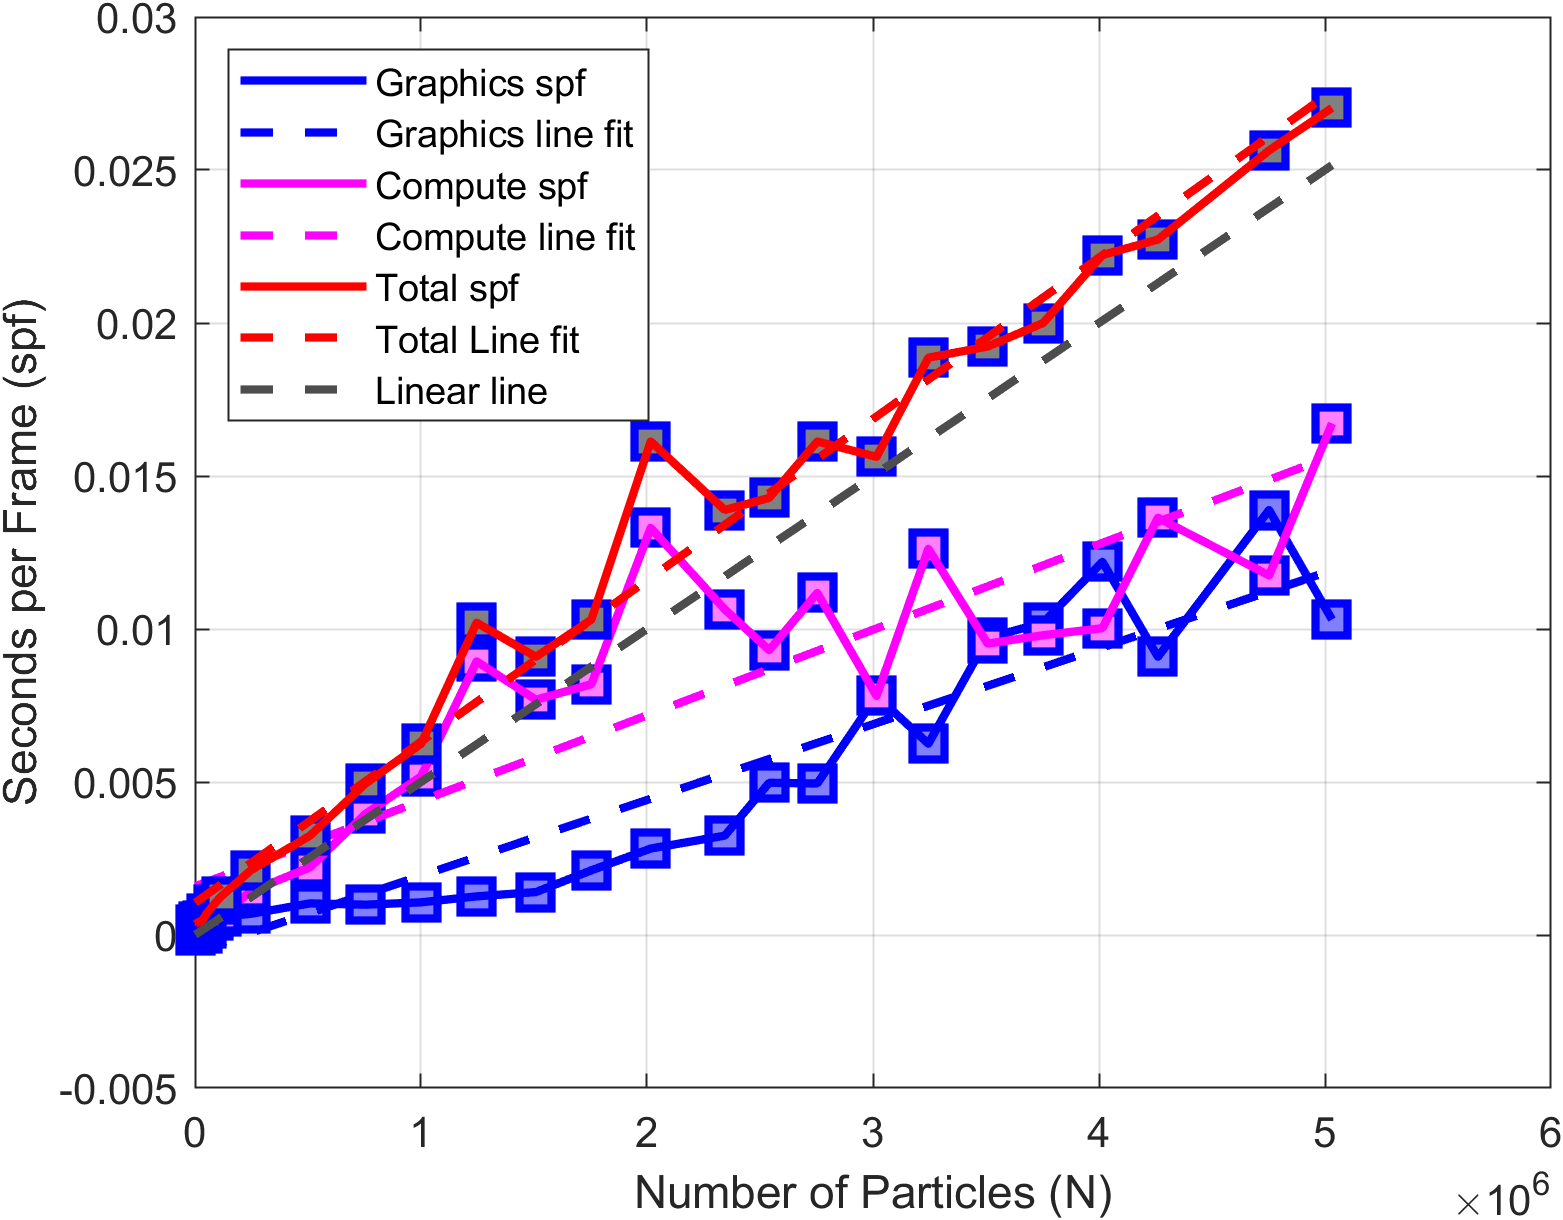
\includegraphics[width=2.97in]{../plots/Perf_VCUBE021.png}
\captionof{figure}[FPS Performance Data]{Seconds per frame for 0.5 collision density with 30 particles per cell verses number of particles.}
\label{fig:Perf_VCUBE02}
\end{figure}

\begin{figure}[h]
\centering
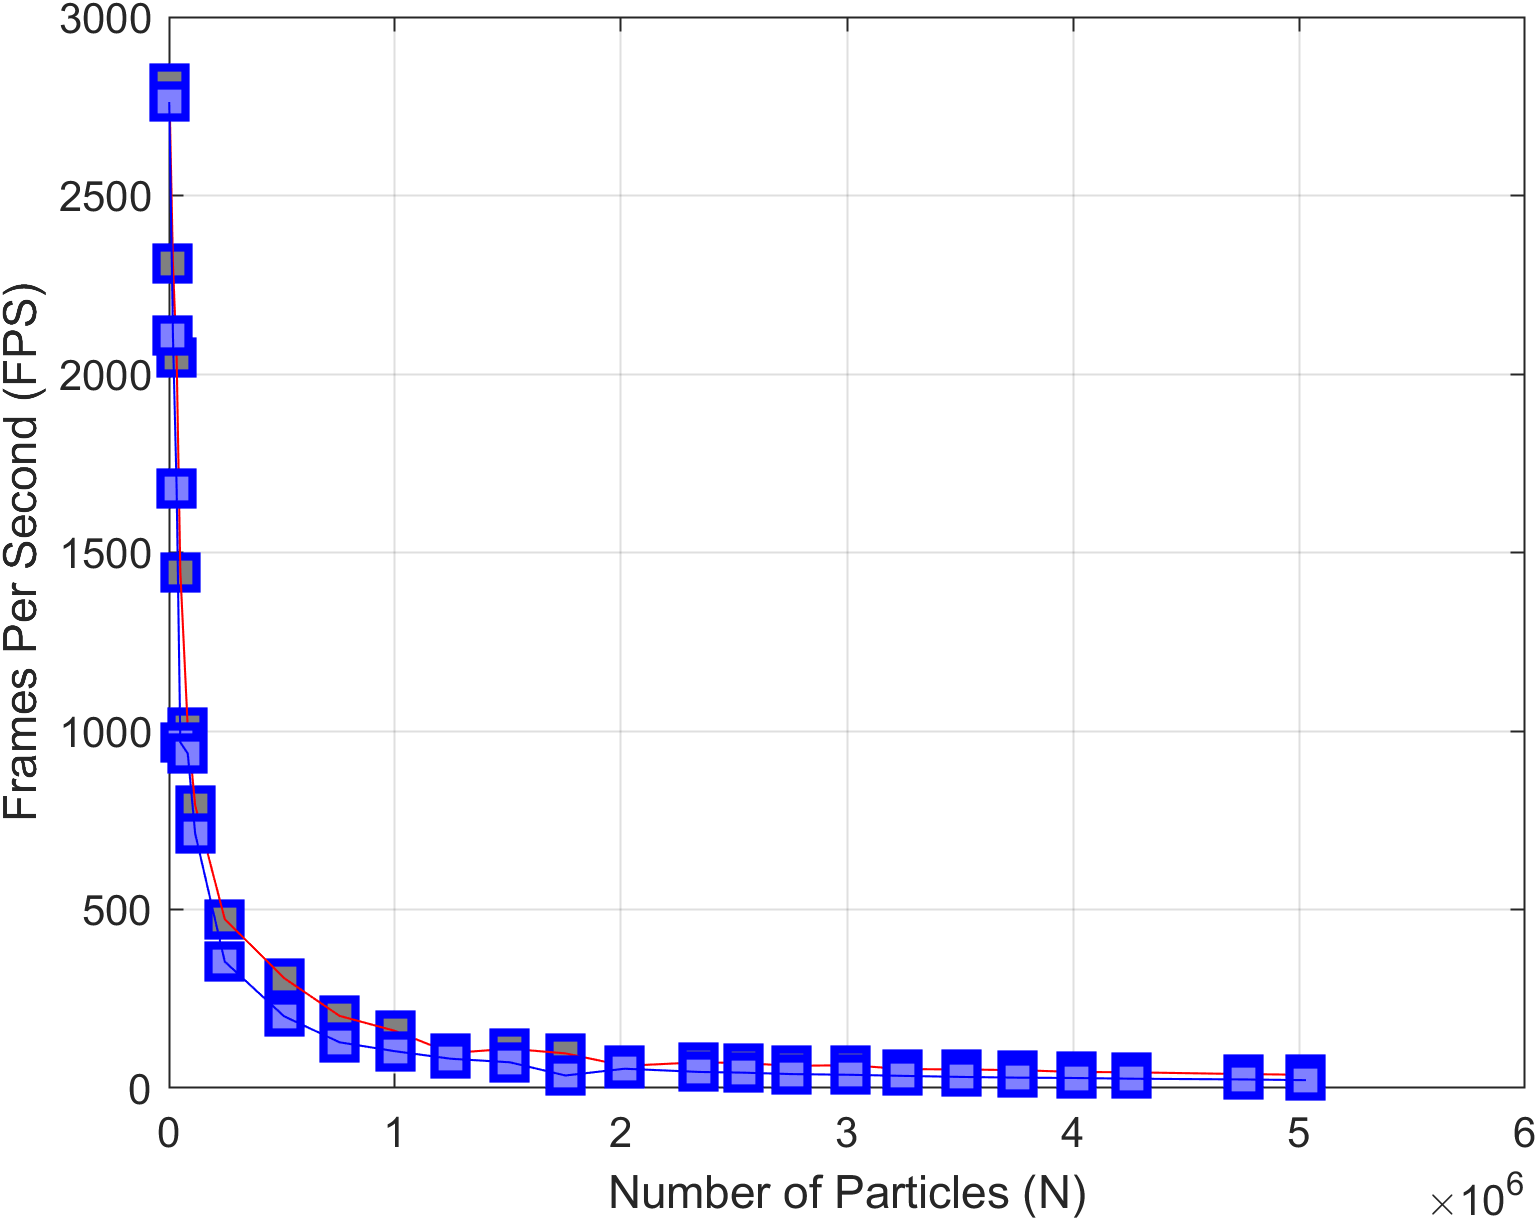
\includegraphics[width=2.97in]{../plots/Perf_VCUBE011.png}
\captionof{figure}[SPf Performance Data]{Frames per second for 0.5 collision density with 30 particles per cell verses number of particles.}
\label{fig:Perf_VCUBE01}
\end{figure}

%\newpage
%\input{../tables/V-Cube Performance Data.tex}
%\newpage
%\input{../tables/V-Cube Performance Data001.tex}
%\newpage
%\begin{figure}[h]
\centering
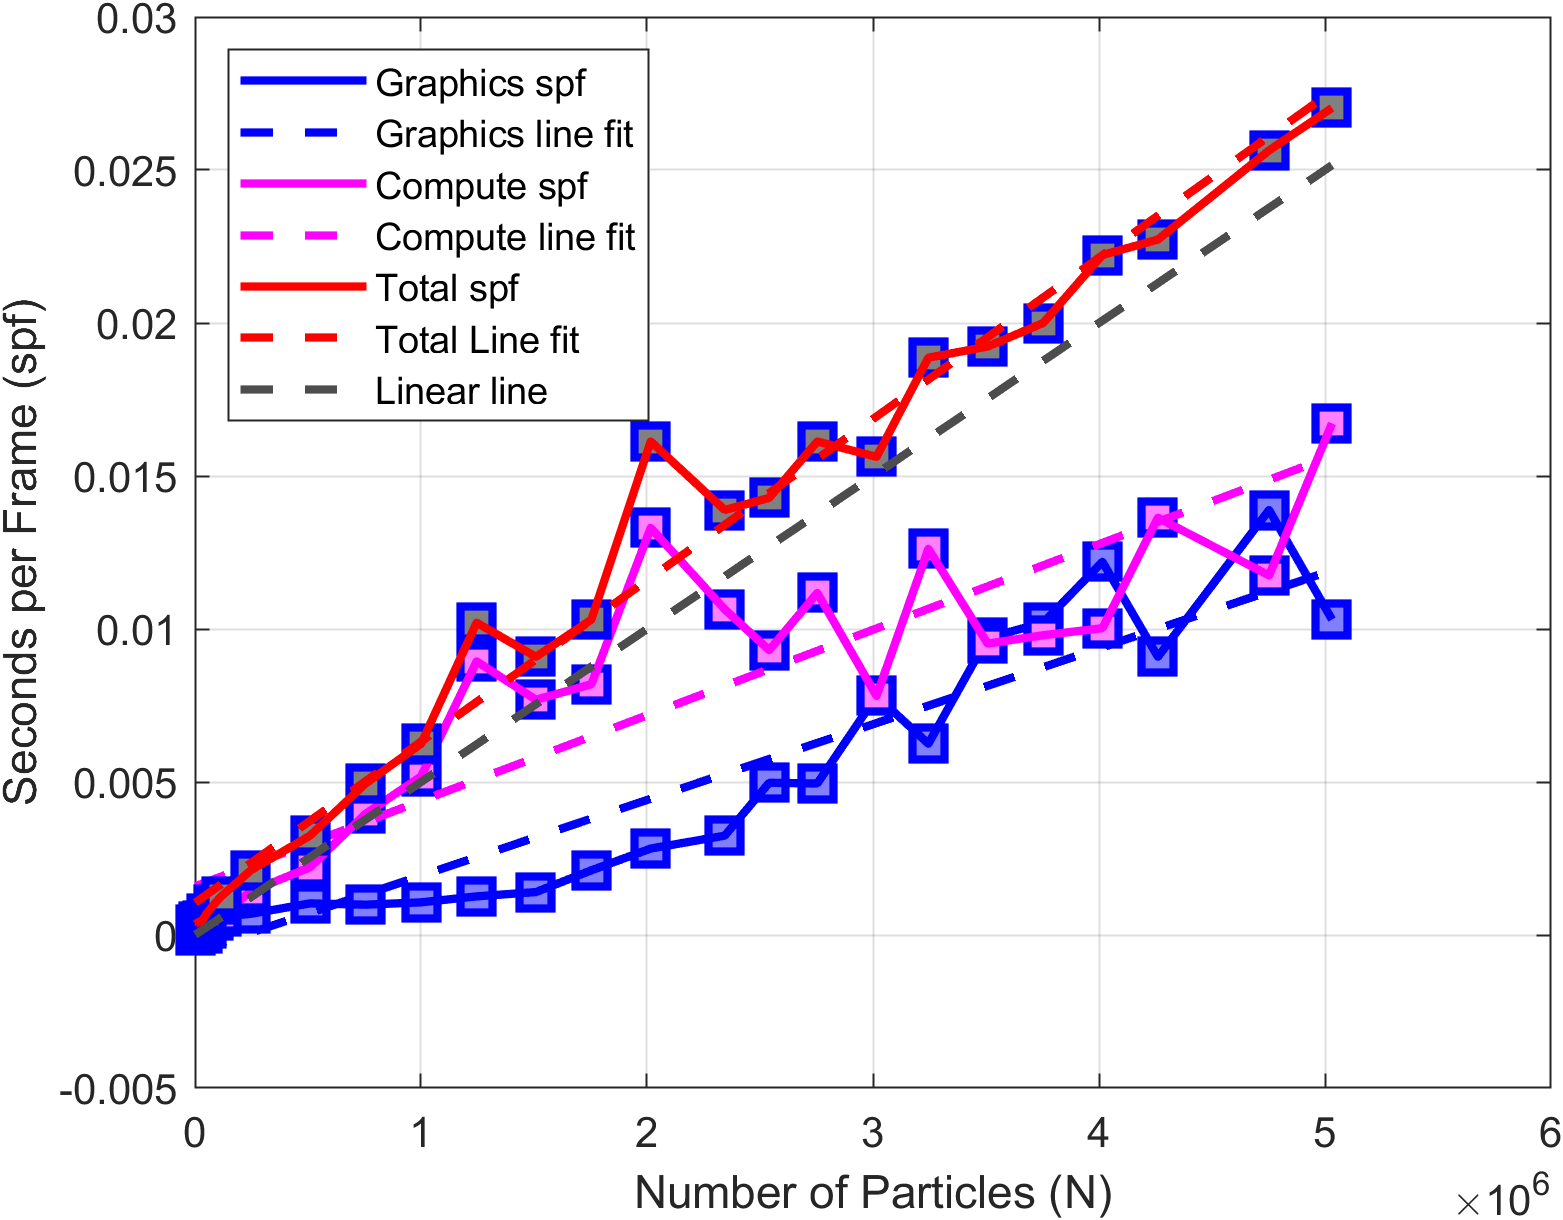
\includegraphics[width=2.97in]{../plots/Perf_VCUBE021.png}
\captionof{figure}[FPS Performance Data]{Seconds per frame for 0.5 collision density with 30 particles per cell verses number of particles.}
\label{fig:Perf_VCUBE02}
\end{figure}

%\begin{figure}[h]
\centering
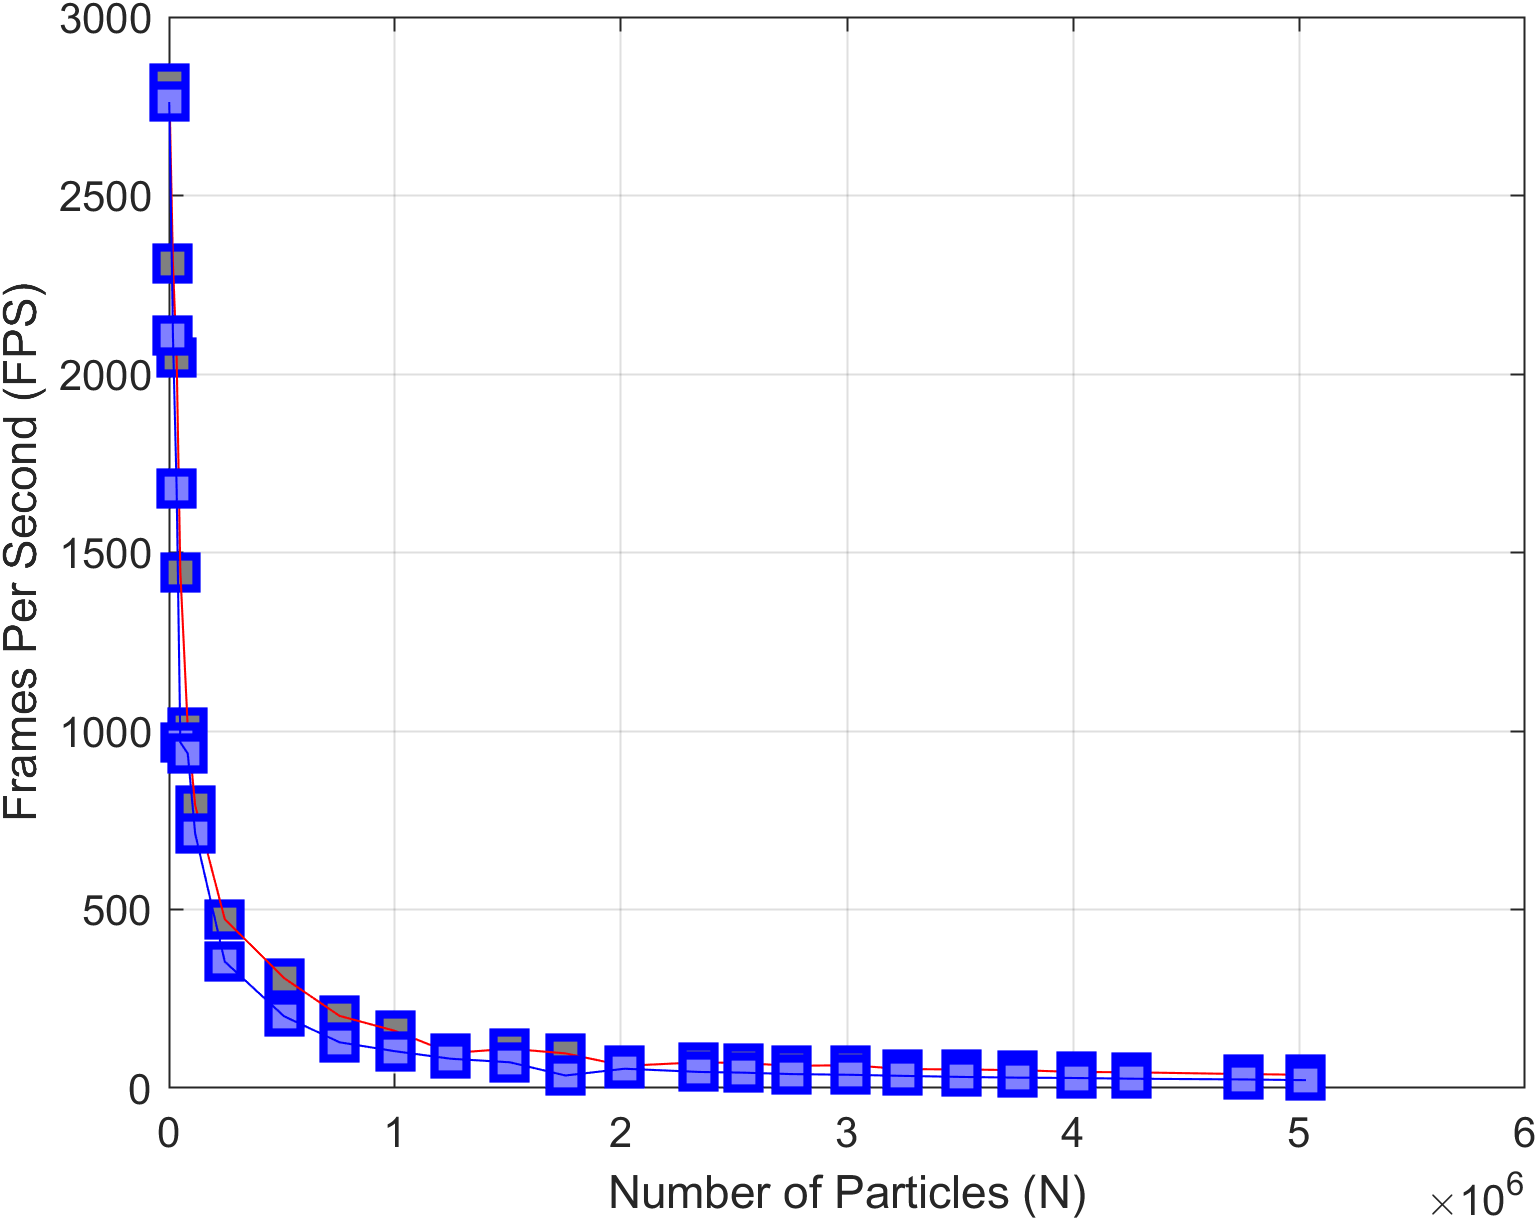
\includegraphics[width=2.97in]{../plots/Perf_VCUBE011.png}
\captionof{figure}[SPf Performance Data]{Frames per second for 0.5 collision density with 30 particles per cell verses number of particles.}
\label{fig:Perf_VCUBE01}
\end{figure}


%\begin{figure}[h]
\centering
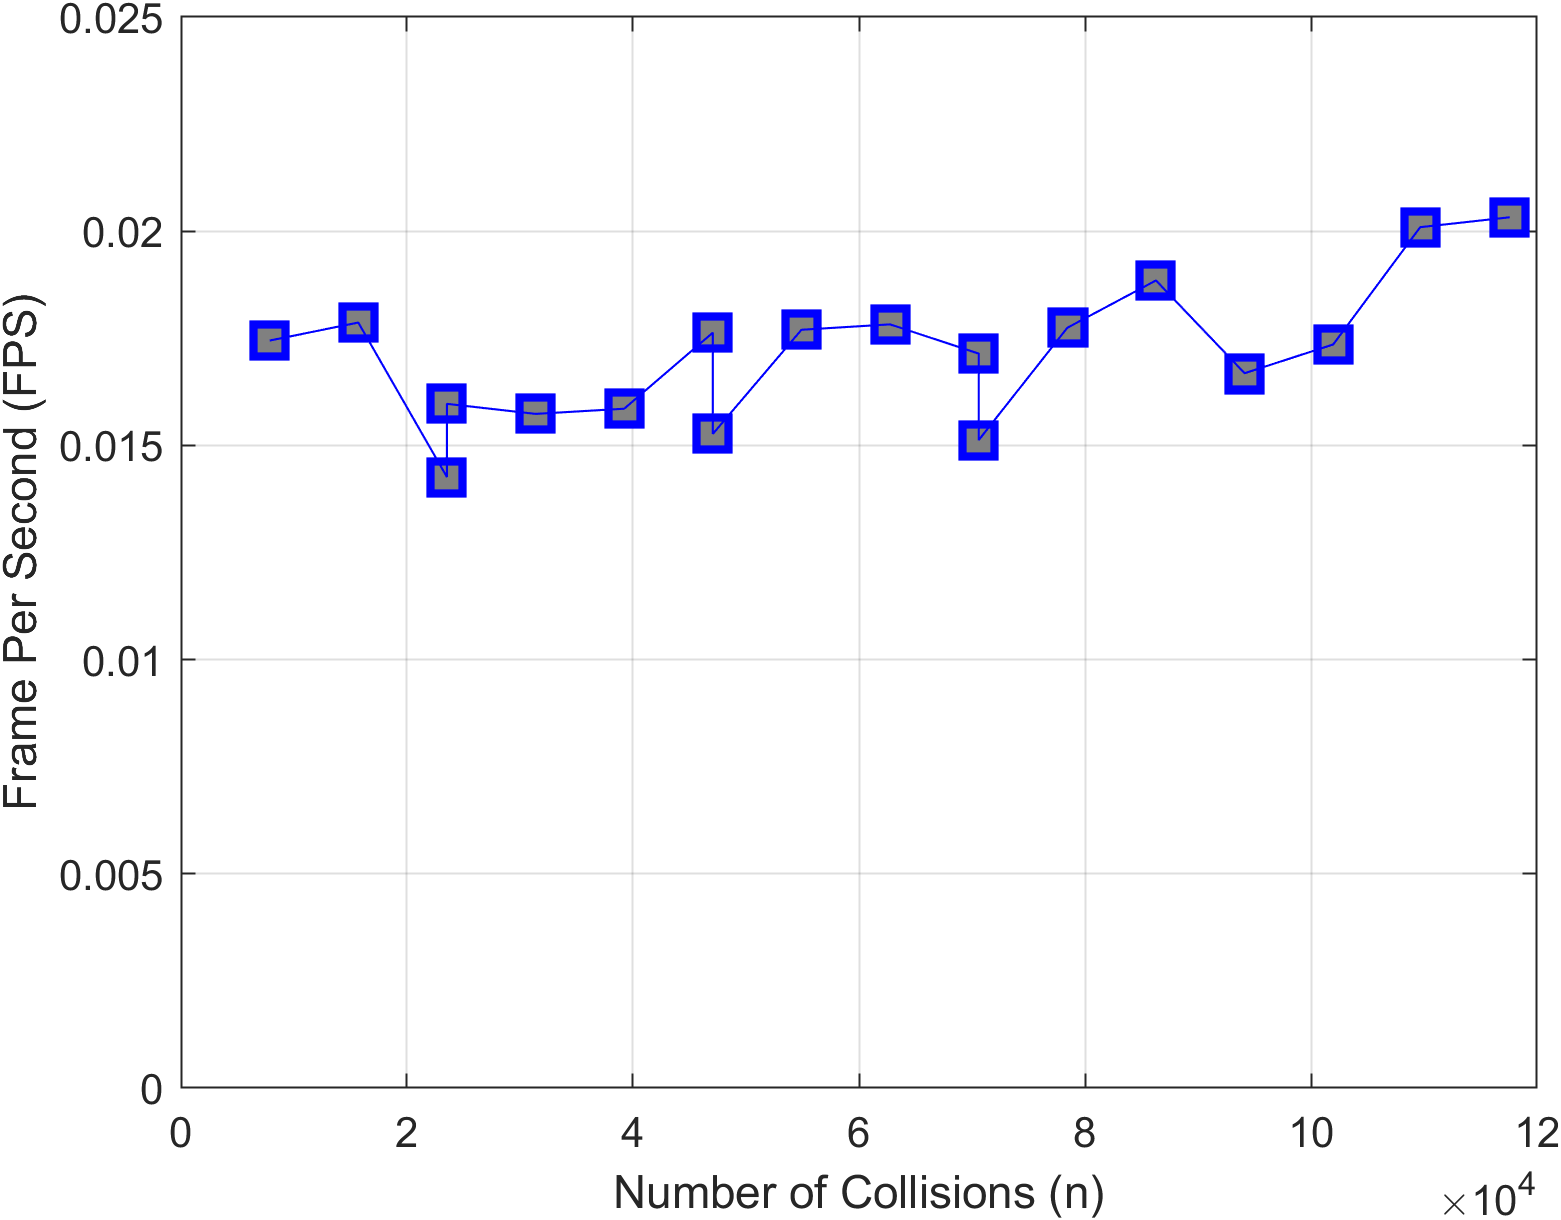
\includegraphics[width=2.97in]{../plots/Perf_RCPCD_Density0011.png}
\captionof{figure}[Frame rate verses density of collisions at 117,650 particles particles and density 0.1-1.0..]{Frame rate verses density of collisions at 117,650 particles and density from 10-100\%}
\label{fig:Perf_RCPCD_Density001}
\end{figure}


%\begin{figure}[h]
\centering
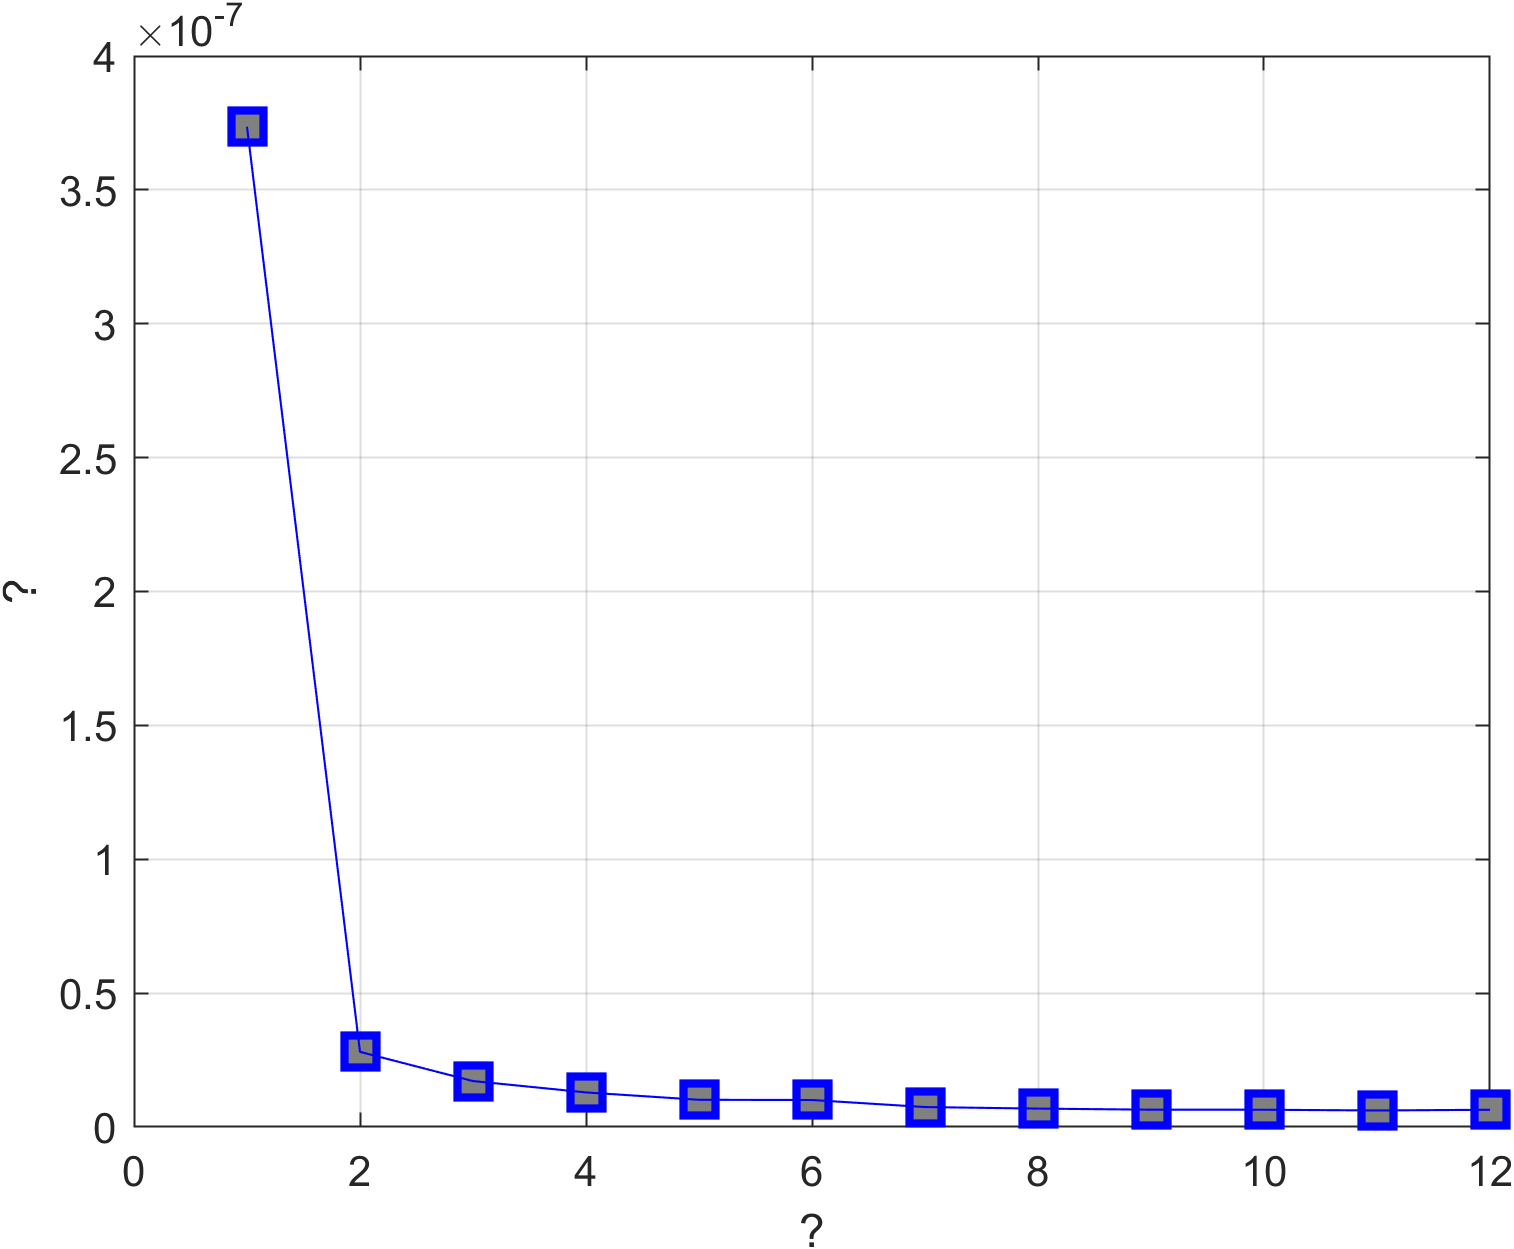
\includegraphics[width=2.97in]{../plots/Perf_VCUBE031.png}
\captionof{figure}[Linearity.]{Linearity - Frame time divided by number of particles for 0.5 collision density with 30 particles per cell verses number of particles.}
\label{fig:Perf_VCUBE03}
\end{figure}


%\begin{figure}[h]
\centering
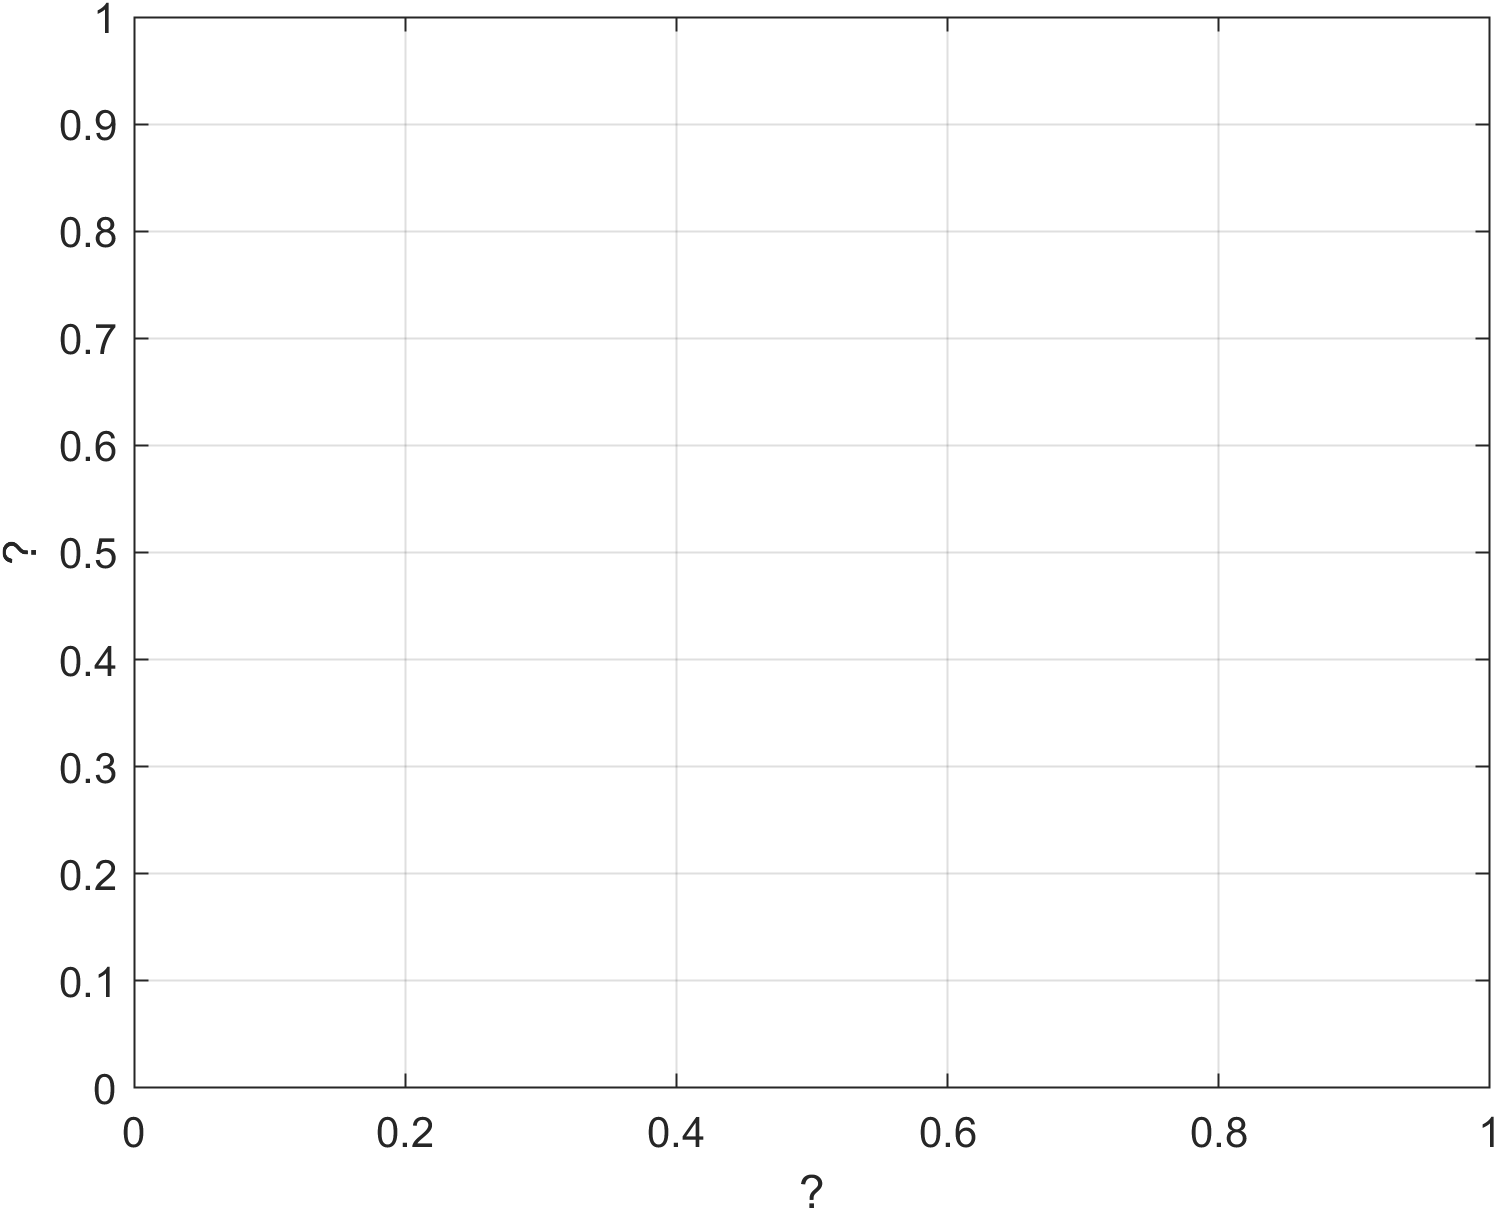
\includegraphics[width=2.97in]{../plots/Perf_VCUBE041.png}
\captionof{figure}[Frame time divided by number of particles.]{CCP number of collisions divided by number of particles for 0.5 collision density with 30 particles per cell verses number of particles.}
\label{fig:Perf_VCUBE04}
\end{figure}

%Fig. \ref{fig:Perf_RCPCD_Density001}

